\documentclass{article}

\usepackage{graphicx}
\usepackage{tikz}
\usepackage{tikzsymbols}
\usetikzlibrary{calc,patterns,shapes.geometric}
\pagestyle{empty}
\usepackage[margin=0pt]{geometry}
\geometry{papersize={14in,12in}}

\def\centerarc[#1](#2)(#3:#4:#5){\draw[#1] ($(#2)+({#5*cos(#3)},{#5*sin(#3)})$) arc (#3:#4:#5);}

\begin{document}
	\begin{figure}
		\centering
		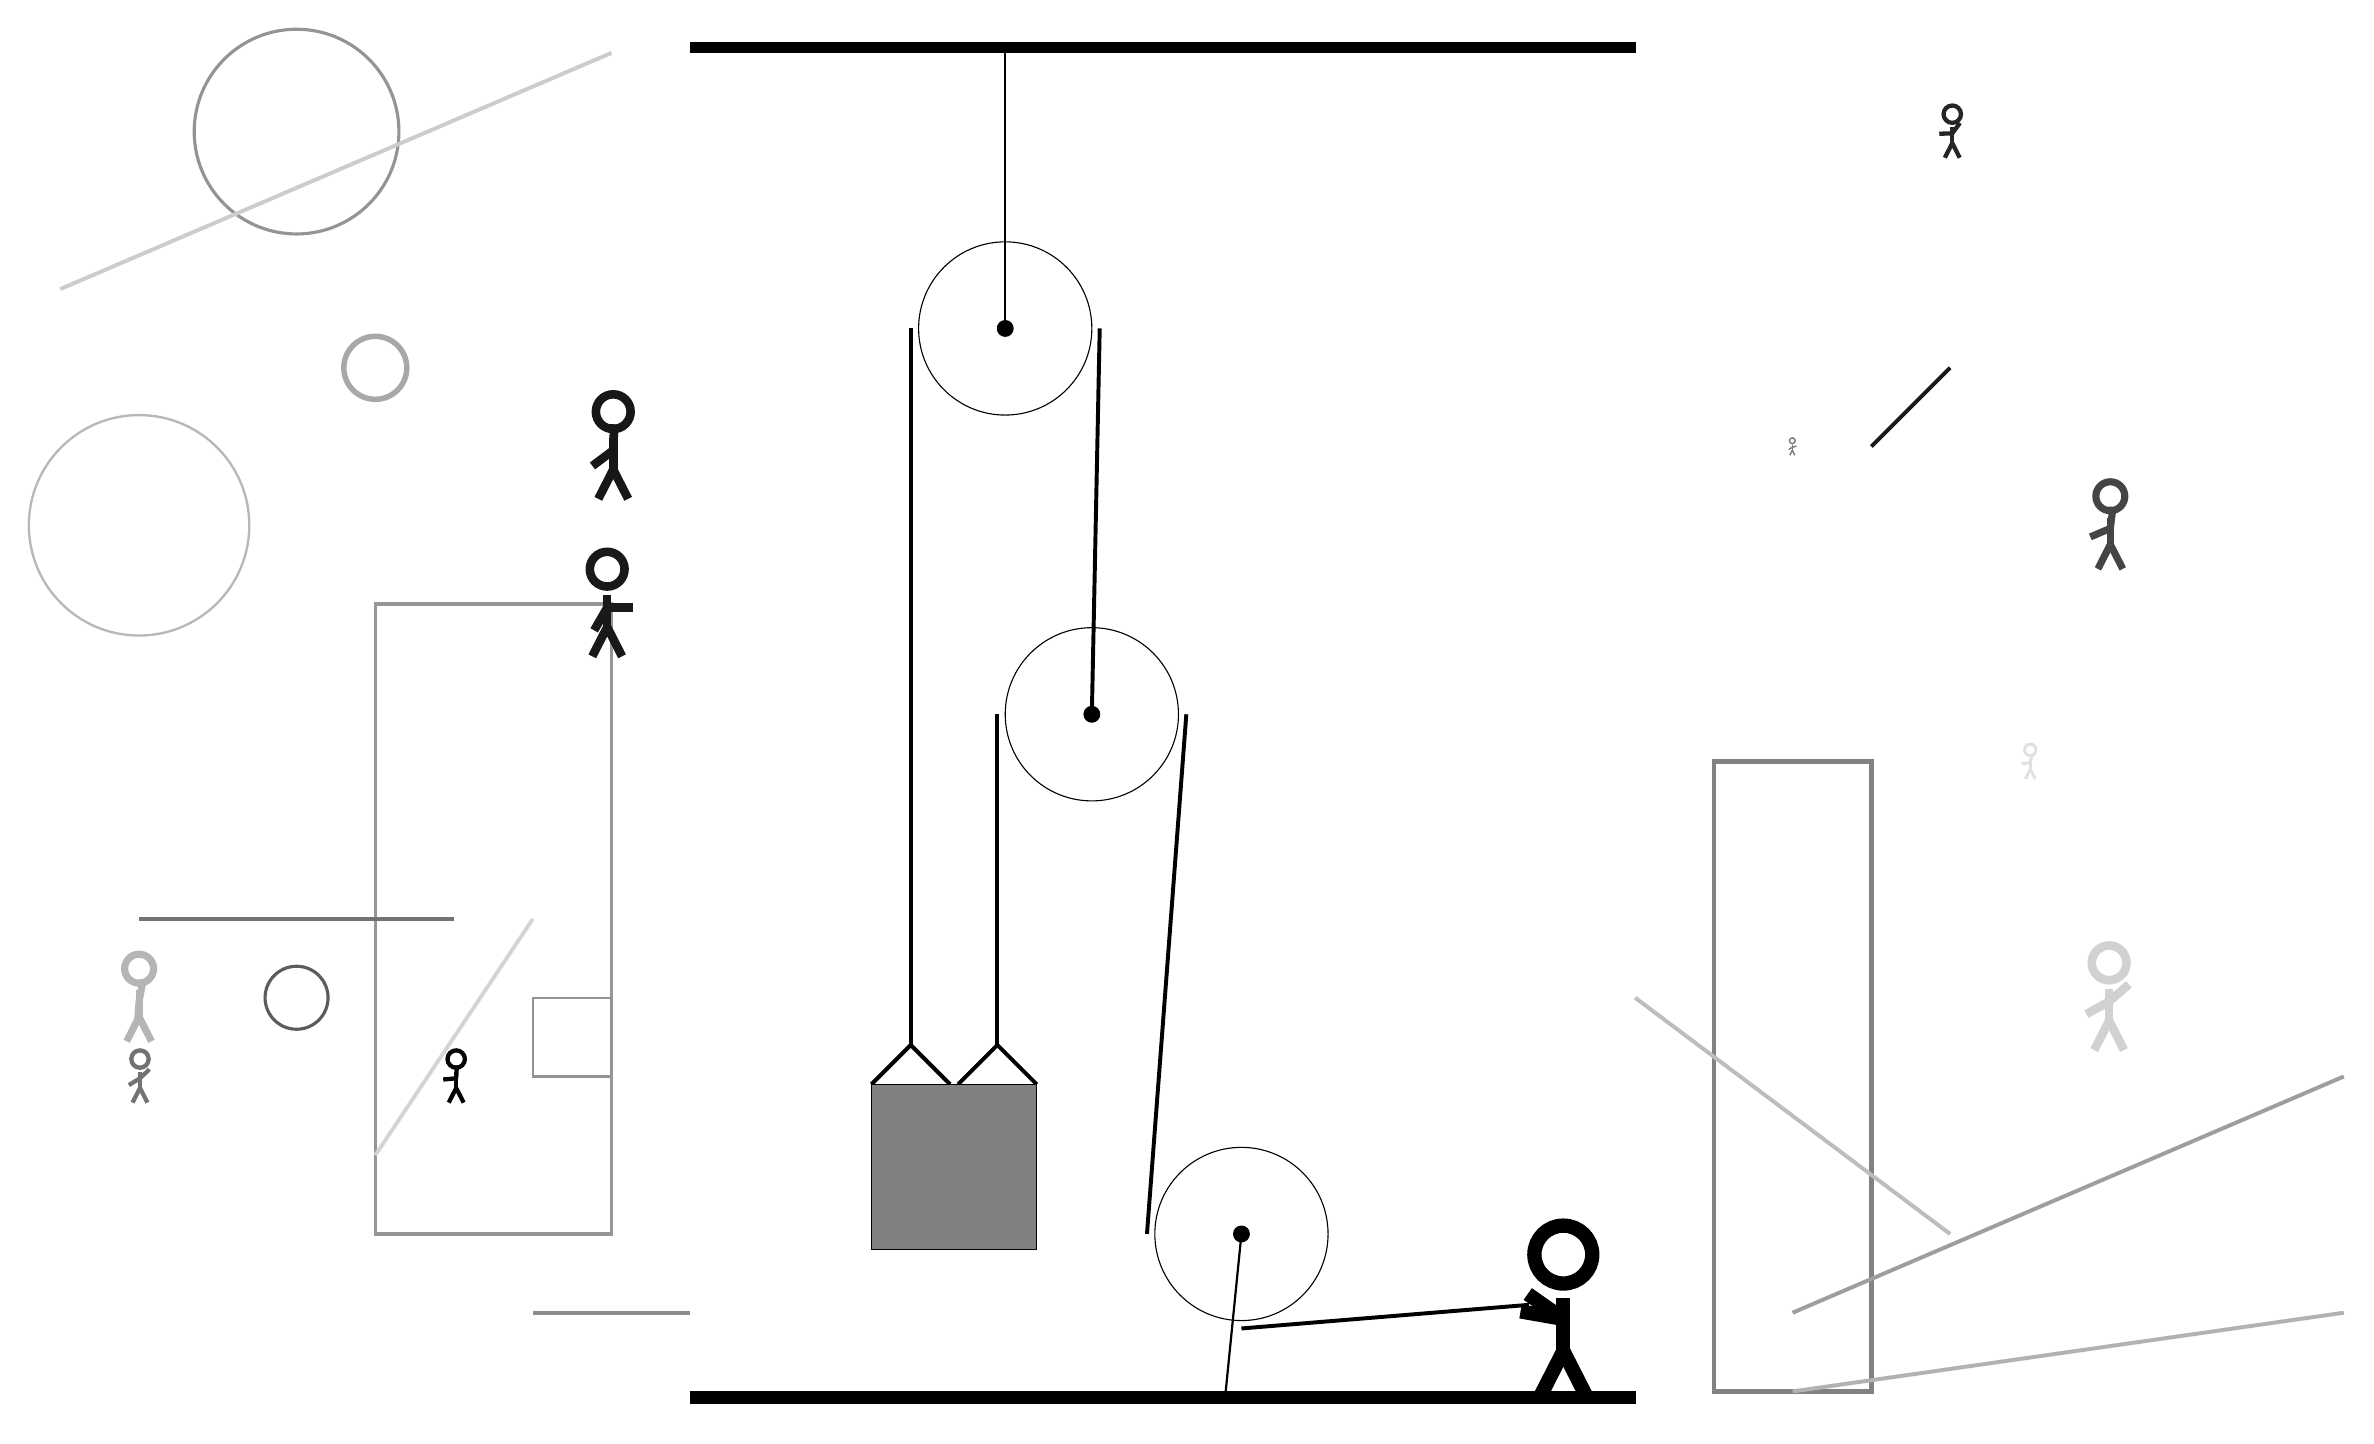
\begin{tikzpicture}
			%%%%% START %%%%%
			
			\draw[fill=black] (-2, 14) rectangle (10, 14.125);
			
			\draw (2, 10.5) circle (1.1);
			\draw[fill=black] (2, 10.5) circle (0.1);
			\draw[thick] (2, 10.5) -- (2, 14);
			
			\draw (3.1, 5.6) circle (1.1);
			\draw[fill=black] (3.1, 5.6) circle (0.1);
			
			\draw (5, -1) circle (1.1);
			\draw[fill=black] (5, -1) circle (0.1);
			\draw[thick] (5, -1) -- (4.8, -3);
			
			\draw[line width=0.4mm, color=black!41] (-3, 7) rectangle (-6, -1);
			
			\draw[line width=0.5mm, color=black!17](-4, 3) -- (-6, 0);
			\draw [line width=0.3mm, color=black!28](-9, 8) circle (1.4);
			\draw[line width=0.6mm, color=black!49] (11, 5) rectangle (13, -3);
			
			\node[line width=0.7mm, color=black!29] at (-9, 2) {\Strichmaxerl[5][86][79]};
			
			\draw[line width=0.3mm, color=black!42] (-3, 2) rectangle (-4, 1);
			\draw[line width=0.5mm, color=black!38](12, -2) -- (19, 1);
			\draw[line width=0.5mm, color=black!45](-4, -2) -- (-2, -2);
			\node[line width=0.6mm, color=black!98] at (-5, 1) {\Strichmaxerl[3][5][87]};
			\draw [line width=0.4mm, color=black!64](-7, 2) circle (0.4);
			\draw [line width=0.4mm, color=black!42](-7, 13) circle (1.3);
			
			\node[line width=0.5mm, color=black!52] at (12, 9) {\Strichmaxerl[1][33][14]};
			\node[line width=0.7mm, color=black!12] at (15, 5) {\Strichmaxerl[2][6][77]};
			
			\node[line width=0.4mm, color=black!91] at (-3, 9) {\Strichmaxerl[6][37][88]};
			\node[line width=0.7mm, color=black!90] at (-3, 7) {\Strichmaxerl[6][60][0]};
			\draw[line width=0.5mm, color=black!20](-3, 14) -- (-10, 11);
			
			\node[line width=0.4mm, color=black!73] at (16, 8) {\Strichmaxerl[5][23][83]};
			
			\draw [line width=0.7mm, color=black!34](-6, 10) circle (0.4);
			\node[line width=0.5mm, color=black!85] at (14, 13) {\Strichmaxerl[3][1][54]};
			
			\draw[line width=0.5mm, color=black!55](-5, 3) -- (-9, 3);
			\node[line width=0.6mm, color=black!55] at (-9, 1) {\Strichmaxerl[3][31][44]};
			
			\draw[line width=0.5mm, color=black!90](14, 10) -- (13, 9);
			\node[line width=0.2mm, color=black!18] at (16, 2) {\Strichmaxerl[6][29][41]};
			\draw[line width=0.5mm, color=black!30](12, -3) -- (19, -2);
			\draw[line width=0.5mm, color=black!26](10, 2) -- (14, -1);
			
			
			\draw[line width = 0.5mm]  (0.3, 0.9) -- (0.8, 1.4) -- (1.3, 0.9);
			\draw[line width = 0.5mm]  (1.4, 0.9) -- (1.9, 1.4) -- (2.4, 0.9);
			\draw[fill=black!50] (0.3, 0.9) rectangle (2.4, -1.2);
			
			\draw[line width = 0.5mm] (0.8, 10.5) -- (0.8, 1.4);
			\centerarc[line width = 0.5mm](2, 10.5)(0:180:1.2000000000000002);
			\draw[line width = 0.5mm] (3.2, 10.5) -- (3.1, 5.6);
			\draw[line width = 0.5mm] (1.9, 5.6) -- (1.9, 1.4);
			\centerarc[line width = 0.5mm](3.1, 5.6)(0:180:1.2000000000000002);
			\draw[line width = 0.5mm] (4.3, 5.6) -- (3.8, -1);
			\centerarc[line width = 0.5mm](5, -1)(180:270:1.2000000000000002);
			\draw[line width = 0.5mm] (5, -2.2) -- (8.65, -1.9);
			
			\node at (9, -2) {\Strichmaxerl[10][-35][170]};
			
			\draw[fill=black] (-2, -3) rectangle (10, -3.15);
			
			%%%%% END %%%%%
		\end{tikzpicture}
	\end{figure}	
\end{document}